\documentclass[10pt,twocolumn]{article}
\usepackage[margin=0.8in,top=0.75in,bottom=0.8in,columnsep=0.28in]{geometry}
\usepackage[T1]{fontenc}
\usepackage{times}
\usepackage{microtype}
\usepackage{graphicx,booktabs,amsmath,array,listings,url}
\lstset{basicstyle=\ttfamily\scriptsize,mathescape=true,columns=fullflexible,keepspaces=true,xleftmargin=2pt,aboveskip=0pt,belowskip=0pt,lineskip=0.5pt}
\usepackage[font=footnotesize,labelfont=bf,skip=2pt]{caption}
\usepackage{titlesec}
\usepackage{xcolor}
\usepackage[colorlinks,allcolors=blue!50!black]{hyperref}
\titleformat{\section}{\normalsize\bfseries\scshape}{\thesection.}{0.5em}{}
\titlespacing*{\section}{0pt}{5pt}{2pt}
\setlength{\parskip}{0pt}
\setlength{\parindent}{10pt}
\linespread{1.03}
\setlength{\textfloatsep}{5pt plus 1pt minus 1pt}
\setlength{\floatsep}{4pt plus 1pt minus 1pt}
\setlength{\intextsep}{4pt plus 1pt minus 1pt}
\renewcommand{\arraystretch}{0.95}
\pagestyle{plain}

\title{\vspace{-8mm}\large\bfseries Divide-and-Conquer in Practice: Closest Pair of Points and\\Karatsuba Multiplication on Inputs of up to One Million\vspace{-2mm}}
\author{\small Sultan Ahmed (24K-0585), Rayyan Ahmer (24K-0690), Hamza Atif (24K-0594)\\[-1pt]
\footnotesize CS2009 -- Design and Analysis of Algorithms, Fall 2026}
\date{}

\begin{document}
\twocolumn[\maketitle\vspace{-9mm}
\begin{center}\begin{minipage}{0.93\textwidth}\small
\textbf{Abstract.} We implement two classic divide-and-conquer algorithms in C++: the $O(n\log n)$ closest pair of points in the plane and Karatsuba's integer multiplication with a schoolbook cut-off. Both were tested on twenty reproducible, seeded input files, from 101 up to $10^6$ points or digits, including adversarial layouts such as duplicates, collinear points, grids and numbers made of zeros. Every answer was checked by at least one independent method, and by an exact comparison wherever feasible. A million points are processed in about 0.27\,s and two million-digit integers are multiplied in about 1.4\,s. Measured growth matches the theory, and a browser interface animates small inputs step by step.
\end{minipage}\end{center}\vspace{1mm}]

\section{Introduction}
Divide and conquer splits a problem into smaller instances, solves them recursively and combines the answers. Its payoff depends on how cheaply the combine step can be done. We study two problems where a clever combine step beats the obvious method. For \emph{closest pair}, brute force checks all $\binom{n}{2}$ pairs, $\Theta(n^2)$, whereas the divide-and-conquer method of Shamos and Hoey~\cite{shamos1975}, presented in Kleinberg and Tardos~\cite{kleinberg2006}, needs only $O(n\log n)$. For \emph{integer multiplication}, the grade-school method costs $\Theta(n^2)$ digit operations, while Karatsuba's trick~\cite{karatsuba1962} replaces four half-size products by three, giving $\Theta(n^{\log_2 3})\approx\Theta(n^{1.585})$.

Our goals are to (i) implement both algorithms without library sorting or big-integer routines, (ii) run them on inputs from 101 points or digits up to $10^6$, (iii) verify every result with independent checks, and (iv) provide an interface that shows the recursion working. The written solutions to the textbook exercises~\cite{levitin2012,kleinberg2006} (min/max, exponentiation, inversions, quicksort, 1-D closest pair) are part of the first submission and are not repeated here.

\section{Proposed System}
Fig.~\ref{fig:sys} shows the architecture, which has three layers, and Fig.~\ref{fig:pseudo} gives the pseudocode of both solvers.

\begin{figure*}[t]
\centering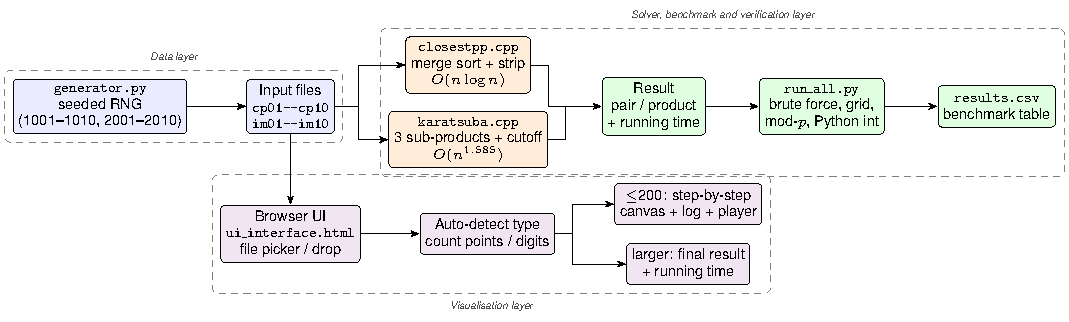
\includegraphics[width=0.98\textwidth]{figures/system.pdf}
\caption{System overview. Seeded files feed the C++ solvers; results are validated by independent checkers and collected in \texttt{results.csv}. The browser UI loads the same files for visualisation.}\label{fig:sys}
\end{figure*}

\begin{figure*}[t]
\centering\footnotesize
\begin{minipage}[t]{0.485\textwidth}
\textbf{Closest pair (Kleinberg--Tardos, Sec.\,5.4)}\vspace{1pt}\hrule\vspace{3pt}
\begin{lstlisting}
CLOSEST(P): sort P by x; return REC(P)
REC(P):   // P sorted by x; returns $\delta$, best pair, P sorted by y
  if |P| $\le$ 3: brute force; sort P by y; return
  $x_m$ $\leftarrow$ x of median point; split P into L, R
  $\delta$ $\leftarrow$ min($\delta_L$, $\delta_R$) from REC(L), REC(R)
  merge L and R by y
  S $\leftarrow$ points with $|x - x_m| < \delta$, in y order
  for each s in S:
    for each later t in S while t.y - s.y < $\delta$:
      if dist(s,t) < $\delta$: update $\delta$ and best pair
  return $\delta$, best pair, P (sorted by y)
\end{lstlisting}\vspace{3pt}\hrule
\end{minipage}\hfill
\begin{minipage}[t]{0.485\textwidth}
\textbf{Karatsuba multiplication}\vspace{1pt}\hrule\vspace{3pt}
\begin{lstlisting}
KARA(x, y):   // limbs in base B = $10^9$
  if x = 0 or y = 0: return 0
  if min(len x, len y) $\le$ 32: return SCHOOL(x, y)
  h $\leftarrow$ ceil(max(len x, len y) / 2)
  x = $x_1 B^h + x_0$;   y = $y_1 B^h + y_0$
  $z_0$ $\leftarrow$ KARA($x_0$, $y_0$)
  $z_2$ $\leftarrow$ KARA($x_1$, $y_1$)
  $z_1$ $\leftarrow$ KARA($x_0{+}x_1$, $y_0{+}y_1$) - $z_0$ - $z_2$
  return $z_2 B^{2h} + z_1 B^h + z_0$
\end{lstlisting}\vspace{3pt}\hrule
\end{minipage}
\caption{Pseudocode of the two implemented algorithms.}\label{fig:pseudo}
\end{figure*}

\textbf{Data layer.} \texttt{generator.py} writes all twenty inputs using one \texttt{random.Random(seed)} per file, so any file can be regenerated alone. Seeds are saved in \texttt{seeds.txt}.

\textbf{Solver layer.} \emph{Closest pair} (\texttt{closestpp.cpp}) first sorts the points by $x$ with our own merge sort. The recursive routine splits the array at the median, solves both halves, and gets $\delta=\min(\delta_L,\delta_R)$. The two halves return sorted by $y$ and are merged, which avoids re-sorting and keeps the combine step linear. Only points with $|x-x_{\text{mid}}|<\delta$ form the strip. Each strip point is compared with its successors in $y$ order until the $y$-gap reaches $\delta$, and a packing argument limits this to a constant number of comparisons. Groups of at most three points use brute force. The recurrence is $T(n)=2T(n/2)+O(n)$, so $T(n)=O(n\log n)$ including the initial sort. \emph{Karatsuba} (\texttt{karatsuba.cpp}) stores numbers as little-endian vectors of base-$10^9$ limbs in 64-bit words. For $x=x_1B^h+x_0$ and $y=y_1B^h+y_0$ it computes $z_0=x_0y_0$, $z_2=x_1y_1$ and $z_1=(x_0+x_1)(y_0+y_1)-z_0-z_2$, and returns $z_2B^{2h}+z_1B^h+z_0$. When the shorter operand has at most 32 limbs (288 digits) it switches to schoolbook multiplication. The recurrence is $T(n)=3T(n/2)+O(n)$, giving $\Theta(n^{\log_2 3})$. Zero operands are trimmed to the empty number, so zero halves cost nothing. Both programs accept \texttt{--check} and \texttt{--trace}, the latter printing one JSON line per divide/combine event for small inputs.

\textbf{Verification and UI layers.} \texttt{run\_all.py} runs every file and checks it as described in Section~\ref{sec:setup}. The interface (\texttt{ui\_interface.html}) is a single self-contained page: the user picks or drops any \texttt{cp*.txt} or \texttt{im*.txt} file, the type is detected automatically, and the matching algorithm runs in the browser. Inputs of up to 200 points or digits are animated with first/previous/play/next/last controls, a canvas (dividing line, strip, best pair; recursion tree and $z_0,z_1,z_2$ for Karatsuba) and a step log. Larger inputs show only the result and the running time.

\section{Experimental Setup}\label{sec:setup}
All programs were compiled with \texttt{g++ -O2 -std=c++17}. Timings are wall-clock \texttt{steady\_clock} values measured around the algorithm itself, which for closest pair includes our merge sort but excludes file reading and writing. One run per file is reported. \textbf{Test machine: a standard consumer laptop (single-threaded runs, no other heavy programs open).} Table~\ref{tab:data} lists every dataset. Coordinates are printed with six decimals, and each integer file holds two decimal numbers on separate lines.

\begin{table}[h]
\centering\footnotesize\setlength{\tabcolsep}{2.5pt}
\caption{Datasets. \texttt{cp}: $n$ points; \texttt{im}: digits per number. Seeds are $1000{+}k$ for \texttt{cp}$k$ and $2000{+}k$ for \texttt{im}$k$.}\label{tab:data}
\begin{tabular}{@{}l r p{5.6cm}@{}}
\toprule
File & Size & Content and generation method\\\midrule
cp01--04 & $10^3$--$10^6$ & Uniform reals in $[0,10^6]^2$\\
cp05 & $10^6$ & 10 random centres, Gaussian noise $\sigma{=}2{\cdot}10^4$, clipped to range\\
cp06 & $10^6$ & Integers in $[0,100]^2$; duplicates, $d{=}0$\\
cp07 & $10^5$ & Same $x{=}500000$, uniform $y$\\
cp08 & $10^5$ & $250{\times}400$ grid, spacing 1000, shuffled\\
cp09 & $10^6$ & Uniform plus a pair at $x_{\text{med}}\pm0.0005$ on one $y$ (crosses split line)\\
cp10 & 101 & Uniform in $[0,1000]^2$, 2 decimals (demo)\\\midrule
im01--04 & $10^3$--$10^6$ & Uniform random digits, no leading zero\\
im05 & $10^6$, 10 & Random digits, very different lengths\\
im06 & $10^5$ & $99\ldots9$ times a random number\\
im07 & 99\,999 & Odd length; each digit is 0 with weight 80, others 3 (about 75\% zeros)\\
im08 & $10^6$ & Both numbers equal $10^{999999}$\\
im09 & $1$, $10^6$ & One number is 0\\
im10 & 101 & Random digits (demo)\\\bottomrule
\end{tabular}
\end{table}

\textbf{Correctness checks.} Closest pair: (a) the reported pair must have the reported distance; (b) an independent uniform-grid method with cell size $\delta$ must find no closer pair (all files); (c) $O(n^2)$ brute force for $n\le 20{,}000$. Multiplication: (a) $(ab)\bmod p=(a\bmod p)(b\bmod p)\bmod p$ for $p=10^9{+}7$ and $998244353$ (all files); (b) exact comparison with Python's \texttt{int} for up to 200{,}000 digits.

\textbf{Reproducibility.} The code, seeds, generator and interface are in the project repository (\url{https://github.com/Syed-56/ProjectAlgoAnalysis}). Running \texttt{generator.py} regenerates all files, and \texttt{run\_all.py} rebuilds \texttt{results.csv}. Files below 1\,MB are submitted, and the larger ones are regenerated from the recorded seeds.

\section{Results and Discussion}
Tables~\ref{tab:cp} and~\ref{tab:im} give the benchmark results, Fig.~\ref{fig:scale} plots time against size, and Table~\ref{tab:cx} compares the measured growth with theory. The fitted slope of 1.09 for closest pair is what $n\log n$ gives over this range (about 1.10), and 1.52 for Karatsuba is a little below 1.585 because the schoolbook cut-off flattens the curve at small sizes.

\begin{table}[h]
\centering\footnotesize\setlength{\tabcolsep}{3pt}
\caption{Closest pair. Every file passed the grid check; brute force was run where $n\le 20{,}000$ and also passed.}\label{tab:cp}
\begin{tabular}{@{}l r r r@{}}
\toprule
File & $n$ & Distance $\delta$ & Time (ms)\\\midrule
cp01 & 1,000 & 1052.432975 & 0.145\\
cp02 & 10,000 & 97.217605 & 1.638\\
cp03 & 100,000 & 8.495326 & 20.924\\
cp04 & 1,000,000 & 0.587626 & 267.319\\
cp05 & 1,000,000 & 0.000021 & 240.841\\
cp06 & 1,000,000 & 0 & 185.442\\
cp07 & 100,000 & 0.000060 & 16.214\\
cp08 & 100,000 & 1000 & 16.017\\
cp09 & 1,000,000 & 0.001000 & 261.548\\
cp10 & 101 & 5.642384 & 0.013\\\bottomrule
\end{tabular}
\end{table}

\begin{table}[h]
\centering\footnotesize\setlength{\tabcolsep}{3pt}
\caption{Karatsuba. Mod-$p$ check passed on all files; exact check against Python \texttt{int} passed where run (Y).}\label{tab:im}
\begin{tabular}{@{}l r r r c@{}}
\toprule
File & Digits & Product digits & Time (ms) & Exact\\\midrule
im01 & 1,000 & 1,999 & 0.038 & Y\\
im02 & 10,000 & 19,999 & 1.144 & Y\\
im03 & 100,000 & 200,000 & 38.839 & Y\\
im04 & 1,000,000 & 2,000,000 & 1361.753 & --\\
im05 & $10^6\times10$ & 1,000,010 & 1.182 & --\\
im06 & 100,000 & 200,000 & 39.831 & Y\\
im07 & 99,999 & 199,998 & 38.338 & Y\\
im08 & 1,000,000 & 1,999,999 & 25.800 & --\\
im09 & $1\times10^6$ & 1 & 0.002 & --\\
im10 & 101 & 202 & 0.003 & Y\\\bottomrule
\end{tabular}
\end{table}


\begin{table}[t]
\centering\footnotesize\setlength{\tabcolsep}{2.2pt}
\caption{Brute force versus divide and conquer (D\&C), theory versus measurement. The measured exponent is the log--log slope between $n{=}10^3$ and $10^6$.}\label{tab:cx}
\begin{tabular}{@{}l l l l c@{}}
\toprule
Problem & Brute force & D\&C & Recurrence & Measured\\\midrule
Closest pair & $\Theta(n^2)$ & $O(n\log n)$ & $2T(\tfrac n2){+}O(n)$ & 1.09\\
Multiplication & $\Theta(n^2)$ & $\Theta(n^{1.585})$ & $3T(\tfrac n2){+}O(n)$ & 1.52\\\bottomrule
\end{tabular}
\end{table}

\begin{figure}[t]
\centering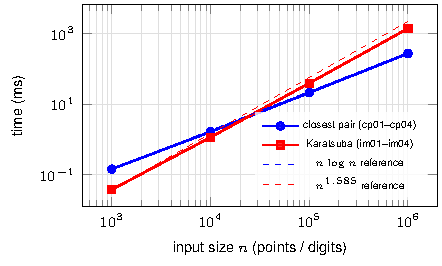
\includegraphics[width=\columnwidth]{figures/scaling.pdf}
\caption{Running time versus input size (log--log) with theoretical reference curves scaled to the first point.}\label{fig:scale}
\end{figure}

\textbf{Closest pair.} Each tenfold increase in $n$ multiplied the time by about 11 to 13 (0.145\,ms to 267\,ms over three decades), which is what $n\log n$ predicts (a tenfold larger input costs about 12 to 13 times more), while brute force would grow 100$\times$ per step. The special files behave as intended. Duplicates (cp06) give $\delta=0$ and finish fastest among the million-point files, plausibly because once $\delta=0$ the strip is empty. On the collinear set (cp07) every point lies in every strip, yet the $y$-gap cut-off keeps the work linear (16.2\,ms for $10^5$ points). The grid (cp08) returns exactly the spacing 1000 despite many ties. The planted pair in cp09 straddles the dividing line and is found with $\delta=0.001$, confirming that the combine step catches cross-boundary pairs.

\textbf{Karatsuba.} The times grow by factors of 30, 34 and 35 per decade, close to the ideal $10^{1.585}\approx 38.5$ and far below the factor of 100 expected from schoolbook. Unequal lengths (im05) fall under the cut-off and cost only $O(nm)$, i.e.\ 1.2\,ms. Because zero halves collapse to empty numbers, the powers of ten (im08) take 25.8\,ms and the zero case (im09) is immediate. The all-nines and sparse inputs (im06, im07) take about the same time as random digits of the same size, so the running time does not depend on the digit values themselves. It only drops when whole blocks of limbs are zero, as in im08. Results for im04, im05, im08 and im09 rest on the double modular check only, because the Python comparison was limited to 200{,}000 digits.

\textbf{Limitations.} Timings come from single runs on one machine, so small differences (for example cp07 versus cp08) are within noise. The interface re-implements the algorithms in JavaScript and is meant for demonstration rather than for million-size timing.

\section{Conclusion}
Both algorithms were implemented from scratch and validated on twenty seeded inputs of up to a million points or digits. The measured scaling agrees with $O(n\log n)$ for closest pair and $\Theta(n^{1.585})$ for Karatsuba, edge cases were handled correctly, and the interface shows the divide, conquer and combine steps for small inputs. Future work could replace the fixed cut-off by a tuned one, or add FFT-based multiplication for comparison~\cite{clrs2022}.

{\footnotesize
\bibliographystyle{plain}
\bibliography{refs}}
\end{document}